\chapter{Cargas e Dimensionamento Preliminares para Asa}

\section{Diagrama Vn}
\label{diagramavn}

O Diagrama Vn foi definido a partir da análise de desempenho realizada para definir o ponto de projeto (\autoref{diagramarestricoes}) e a análise aerodinâmica da aeronave (\autoref{superf_sustentadoras}) considernado asa limpa (sem deflexão de superfícies de hipersustentação) e MTOW. A \autoref{tbl:velocidadesprojeto} resume as velocidades de projeto de acordo com Iscold \cite{iscold} e o diagrama vn é apresentado na \autoref{fig:diagramavn} conforme a norma \textit{CFR Part 25}. O fator de carga máximo da aeronave é 2.5 e o fator de carga mínimo é -1.

\begin{figure}[H]
\centering
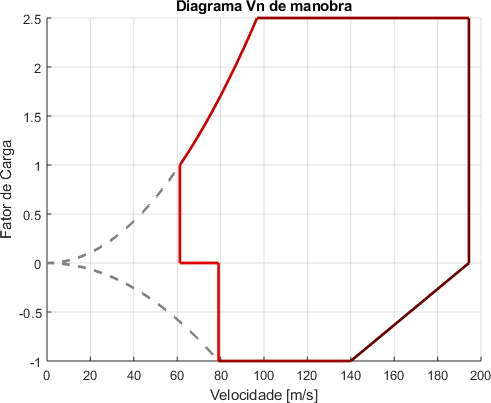
\includegraphics[width=0.75\textwidth]{images/parte3/diagramavn_asalimpa.png}
\caption[Diagrama Vn]{Diagrama Vn}
\label{fig:diagramavn}
\end{figure}

\begin{table}[H]
\centering
\begin{tabular}{cccc}
\toprule
Velocidade & Descrição & Definição & Valor \\ \midrule
$V_{S_{+}}$ & Velocidade de estol & $ \sqrt{\frac{2 W}{\rho S C_{L_{max}}}} $ & 61.33 m/s \\ [0.3cm]
 & positivo (asa limpa) & &  \\ [0.3cm]
$V_A$ & Velocidade de Manobra & $ V_{S_{+}} \sqrt{n_{max}} $ & 96.97 m/s \\ [0.3cm]
$V_C$ & Velocidade de Cruzeiro & Requisito & 140 m/s \\  [0.3cm]
$V_H$ & Velocidade Horizontal & $V_C/0.9$ & 155.56 m/s \\  [0.3cm]
 & Máxima & &  \\ [0.3cm]
$V_D$ & Velocidade de Mergulho & $1.25 V_C$ & 194.44 m/s \\ [0.3cm]
$V_{S_{-}}$ & Velocidade de estol & $ \sqrt{\frac{2 W}{\rho S C_{L_{min}}}} $ & 79.17 m/s \\ [0.3cm]
 & negativo (asa limpa) & &  \\ [0.3cm]
\bottomrule
\end{tabular}
\caption[Velocidades de Projeto - Asa Limpa]{Velocidades de Projeto - Asa Limpa}
\label{tbl:velocidadesprojeto}
\end{table}

\clearpage

\section{Cargas Preliminares}

Uma verificação da longarina da asa é necessária visto que o caixão tem sua altura limitada pela espessura máximo do perfil sendo assim diretamente impactado pela escolha da perfilagem da asa. Na análise realizada na \autoref{perfilasa}, procurou-se desde o início considerar perfis com espessura relativa acima de 12\% para previnir possíveis problemas estruturais. Dessa forma, a verificação estrutural foi realizada para garantir que o perfil escolhido não prejudique o projeto estrutural.

O cálculo de cargas precede a avaliação da estrutura e portanto foi realizado uma estimativa preliminar considerando o diagrama Vn apresentando na \autoref{diagramavn}. Considerou-se o extremo do diagrama Vn na condição de velocidade de mergulho e fator de carga máximo para cálculo das cargas aerodinâmicas pois espera-se que essa condição seja crítica para cargas estáticas. Além disso, cargas inerciais não foram consideradas pois estas tendem a aliviar as cargas aerodinâmicas em condições estáticas e visto que a análise é preliminar, decidiu-se fazer uma estimativa conservadora sem considerar o peso próprio da asa e do motor.

Para trimagem da aeronave na condição crítica escolhida, considerou-se o profundor definido na análise de estabilidade no \autoref{estabilidade} e as polares apresentadas na \autoref{superf_sustentadoras}. O ângulo de ataque da asa estimado para esta condição foi de 0.5 \textdegree\ e com esse valor foi possível estimar a distribuição de sutentação da asa a partir do software CEA-VLM. As figuras abaixo apresentam a sustentação e as cargas aerodinâmicas integradas pela envergadura.

\begin{figure}[H]
\centering
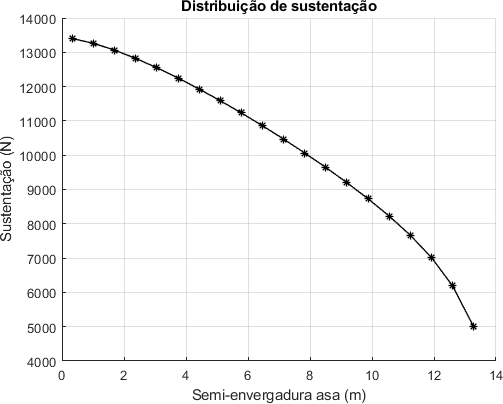
\includegraphics[width=0.65\textwidth]{images/parte3/loads_lift.png}
\caption{Distribuição da Sustentação}
\label{fig:loads_lift}
\end{figure}

\begin{figure}[H]
\centering
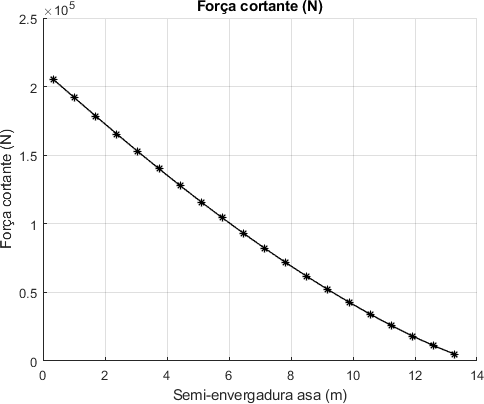
\includegraphics[width=0.65\textwidth]{images/parte3/loads_shear.png}
\caption{Cargas integradas: esforços cortante}
\label{fig:loads_shear}
\end{figure}


\begin{figure}[H]
\centering
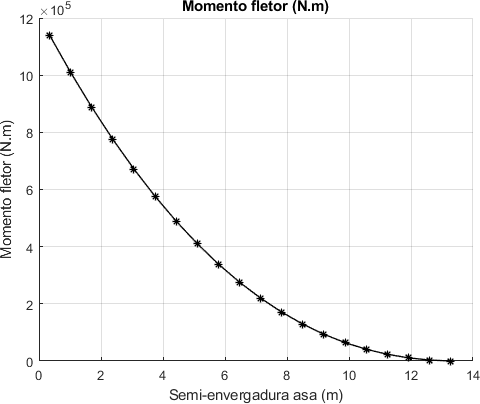
\includegraphics[width=0.65\textwidth]{images/parte3/loads_bending.png}
\caption{Cargas integradas: momento fletor}
\label{fig:loads_bending}
\end{figure}


\clearpage
\section{Dimensionamento Preliminar}

A partir do esforços apresentados nas figuras \ref{fig:loads_shear} e \ref{fig:loads_bending}, pode-se realizar um dimensionamento inicial da estrutura principal da asa, utilizando o momento de inércia de cada seção, o momento fletor atuante e a distância do centro da seção até as extremidades, onde o valor da tensão é maior.

Considerou-se, no primeiro dimensionamento, que as longarinas serão fabricadas de uma liga de alumínio da série 7000 e o valor de tensão obtido em cada seção foi comparado ao limite de resistência do material selecionado. Considerou-se a existência de duas longarinas em perfil C, formando com o revestimento, um caixão principal capaz de suportar os esforços de torção na asa, e considerou-se que as longarinas suportariam sozinhas os esforços fletores. Os resultados obtidos do dimensionamento estrutural das longarinas estão apresentados na \autoref{tbl:longarinas} e foram considerados satisfatórios. Dessa forma a perfilagem da asa não prejudicou o projeto estrutural como desejava-se verificar.


\begin{table}[H]
\centering
\begin{tabular}{ccc}
\toprule
(mm) & Raiz & Ponta \\ \midrule
Longarina 1 &  &   \\ \midrule
Altura mesas & 12 & 8 \\
Largura mesas & 60 & 40\\
Altura alma & 447.6 & 266.6 \\
Largura alma & 5 & 2.5 \\ \midrule
Longarina 2 &  &   \\ \midrule
Altura mesas & 10 & 5 \\
Largura mesas & 50 & 30 \\
Altura alma & 373.0 & 225.5 \\
Largura alma & 5 & 2.5 \\
\bottomrule
\end{tabular}
\caption{Dimensionamento Preliminar da Longarina da Asa}
\label{tbl:longarinas}
\end{table}
